\documentclass{article}\usepackage[]{graphicx}\usepackage[]{color}
%% maxwidth is the original width if it is less than linewidth
%% otherwise use linewidth (to make sure the graphics do not exceed the margin)
\makeatletter
\def\maxwidth{ %
  \ifdim\Gin@nat@width>\linewidth
    \linewidth
  \else
    \Gin@nat@width
  \fi
}
\makeatother

\definecolor{fgcolor}{rgb}{0.345, 0.345, 0.345}
\newcommand{\hlnum}[1]{\textcolor[rgb]{0.686,0.059,0.569}{#1}}%
\newcommand{\hlstr}[1]{\textcolor[rgb]{0.192,0.494,0.8}{#1}}%
\newcommand{\hlcom}[1]{\textcolor[rgb]{0.678,0.584,0.686}{\textit{#1}}}%
\newcommand{\hlopt}[1]{\textcolor[rgb]{0,0,0}{#1}}%
\newcommand{\hlstd}[1]{\textcolor[rgb]{0.345,0.345,0.345}{#1}}%
\newcommand{\hlkwa}[1]{\textcolor[rgb]{0.161,0.373,0.58}{\textbf{#1}}}%
\newcommand{\hlkwb}[1]{\textcolor[rgb]{0.69,0.353,0.396}{#1}}%
\newcommand{\hlkwc}[1]{\textcolor[rgb]{0.333,0.667,0.333}{#1}}%
\newcommand{\hlkwd}[1]{\textcolor[rgb]{0.737,0.353,0.396}{\textbf{#1}}}%

\usepackage{framed}
\makeatletter
\newenvironment{kframe}{%
 \def\at@end@of@kframe{}%
 \ifinner\ifhmode%
  \def\at@end@of@kframe{\end{minipage}}%
  \begin{minipage}{\columnwidth}%
 \fi\fi%
 \def\FrameCommand##1{\hskip\@totalleftmargin \hskip-\fboxsep
 \colorbox{shadecolor}{##1}\hskip-\fboxsep
     % There is no \\@totalrightmargin, so:
     \hskip-\linewidth \hskip-\@totalleftmargin \hskip\columnwidth}%
 \MakeFramed {\advance\hsize-\width
   \@totalleftmargin\z@ \linewidth\hsize
   \@setminipage}}%
 {\par\unskip\endMakeFramed%
 \at@end@of@kframe}
\makeatother

\definecolor{shadecolor}{rgb}{.97, .97, .97}
\definecolor{messagecolor}{rgb}{0, 0, 0}
\definecolor{warningcolor}{rgb}{1, 0, 1}
\definecolor{errorcolor}{rgb}{1, 0, 0}
\newenvironment{knitrout}{}{} % an empty environment to be redefined in TeX

\usepackage{alltt}
\usepackage{graphicx, color, hyperref, fancyhdr}

%\usepackage{amsmath,amssymb,amsthm}
\usepackage{fancyhdr,url}
\usepackage{graphicx}

\oddsidemargin 0in  %0.5in
\topmargin     0in
\leftmargin    0in
\rightmargin   0in
\textheight    9in
\textwidth     6in %6in
%\headheight    0in
%\headsep       0in
%\footskip      0.5in

\newtheorem{thm}{Theorem}
\newtheorem{cor}[thm]{Corollary}
\newtheorem{obs}{Observation}
\newtheorem{lemma}{Lemma}
\newtheorem{claim}{Claim}
\newtheorem{definition}{Definition}
\newtheorem{question}{Question}
\newtheorem{answer}{Answer}
\newtheorem{problem}{Problem}
\newtheorem{solution}{Solution}
\newtheorem{conjecture}{Conjecture}

\pagestyle{fancy}

\lhead{\textsc{MATH 243}}
\chead{\textsc{Practice}}
\rhead{\textsc{\today}}
\lfoot{}
\cfoot{}
%\cfoot{\thepage}
\rfoot{}
\renewcommand{\headrulewidth}{0.2pt}
\renewcommand{\footrulewidth}{0.0pt}

\newcommand{\ans}{\vspace{0.25in}}

\usepackage[top=.8in, bottom=.5in, left=1.5in, right=1.5in]{geometry}
\thispagestyle{empty}
\IfFileExists{upquote.sty}{\usepackage{upquote}}{}
\begin{document}

\begin{center}
\textsc{Math 243: Statistical Learning} \\
\noindent\rule{12cm}{0.4pt}
\end{center}

\subsection*{Boosted Trees}

\emph{One Weak Learner} ($b = 1$): We'd like to build a boosted tree that will predict a value for $Y$ given $X_1$ and $X_2$ using the 8 training observations found in the table below.

\begin{enumerate}
\item The structure of the first weak learner is shown in the tree diagram below. Please fill in the prediction at each of the leaves as well as in the table in the column labeled $\hat{f}^1(x)$.

\vspace{10mm}

\begin{minipage}[t]{.4\textwidth}
{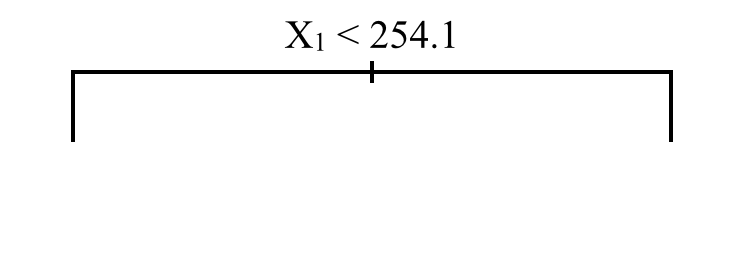
\includegraphics[width=\textwidth]{treeA.png}}
\end{minipage}
\hfill
\begin{minipage}[t]{.4\textwidth}
% latex table generated in R 3.2.3 by xtable 1.8-0 package
% Wed Mar 30 10:02:24 2016
\begin{tabular}{rrrrll}
  \hline
 & $X_1$ & $X_2$ & $Y$ & $\hat{f}^1(x)$ & r \\ 
  \hline
1 & 270.00 & 3.81 & 15.00 &  &  \\ 
  2 & 86.03 & 0.86 & 23.00 &  &  \\ 
  3 & 149.53 & 4.44 & 19.00 &  &  \\ 
  4 & 331.15 & 3.77 & 16.00 &  &  \\ 
  5 & 430.89 & 5.68 & 10.00 &  &  \\ 
  6 & 338.36 & 3.18 & 13.00 &  &  \\ 
  7 & 46.33 & 3.17 & 27.00 &  &  \\ 
  8 & 238.19 & 3.35 & 21.00 &  &  \\ 
   \hline
\end{tabular}

\end{minipage}

\vspace{8mm}
\item Carefully draw the surface corresponding to $\hat{f}^1(x)$ on the 3D scatterplot below.

\vspace{-8mm}

\begin{center}
{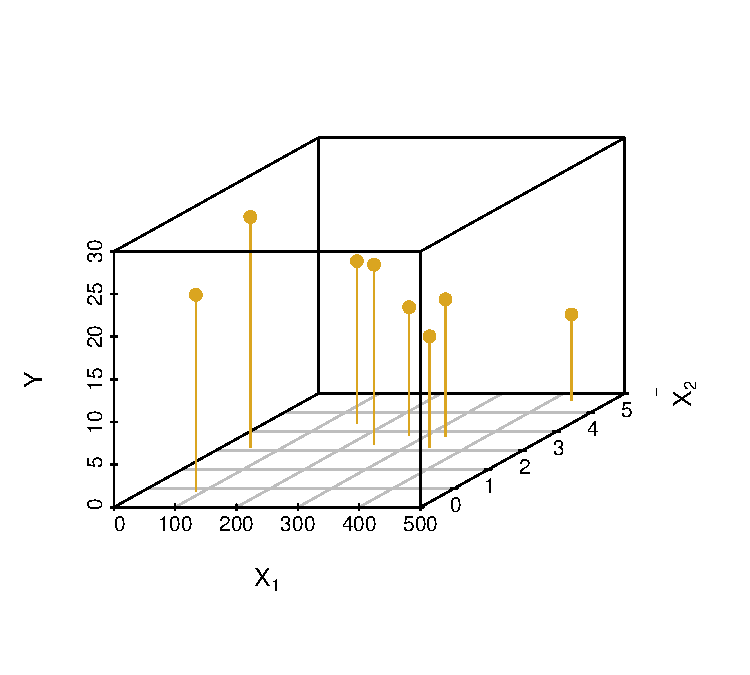
\includegraphics[scale=0.9]{scatterA.pdf}}
\end{center}

\vspace{-8mm}

\item Now that you have the prediction from the weak learner, please compute the residuals for each observation to find out where this learner did well and where it did poorly. Fill them in the column labeled \emph{r}.

\end{enumerate}

\newpage

\begin{center}
\textsc{Math 243: Statistical Learning} \\
\noindent\rule{12cm}{0.4pt}
\end{center}

\subsection*{Boosted Trees}

\emph{Second Weak Learner} ($b = 2$): Now we strengthen our tree by incorporating a second weak learner that addresses the most glaring deficiencies of the first learner.

\begin{enumerate}
\item The structure of the second weak learner is shown in the tree diagram below. Please fill in the prediction at each of the leaves as well as in the table in the column labeled $\hat{f}^2(x)$.

\vspace{10mm}

\begin{minipage}[t]{.4\textwidth}
{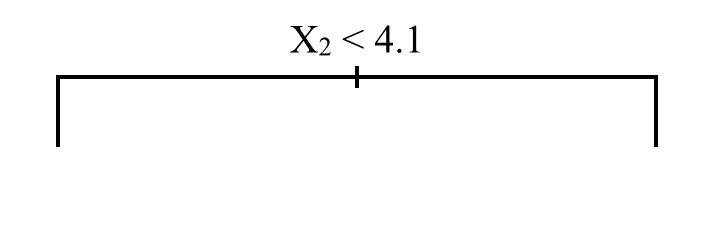
\includegraphics[width=\textwidth]{treeB.png}}
\end{minipage}
\hfill
\begin{minipage}[t]{.4\textwidth}
% latex table generated in R 3.2.3 by xtable 1.8-0 package
% Wed Mar 30 10:02:24 2016
\begin{tabular}{rrrrll}
  \hline
 & $X_1$ & $X_2$ & $r_{old}$ & $\hat{f}^2(x)$ & $r_{new}$ \\ 
  \hline
1 & 270.00 & 3.81 & 1.50 &  &  \\ 
  2 & 86.03 & 0.86 & 0.50 &  &  \\ 
  3 & 149.53 & 4.44 & -3.50 &  &  \\ 
  4 & 331.15 & 3.77 & 2.50 &  &  \\ 
  5 & 430.89 & 5.68 & -3.50 &  &  \\ 
  6 & 338.36 & 3.18 & -0.50 &  &  \\ 
  7 & 46.33 & 3.17 & 4.50 &  &  \\ 
  8 & 238.19 & 3.35 & -1.50 &  &  \\ 
   \hline
\end{tabular}

\end{minipage}

\vspace{8mm}
\item Carefully draw the surface corresponding to $\hat{f}^2(x)$ on the 3D scatterplot below.

\vspace{-8mm}

\begin{center}
{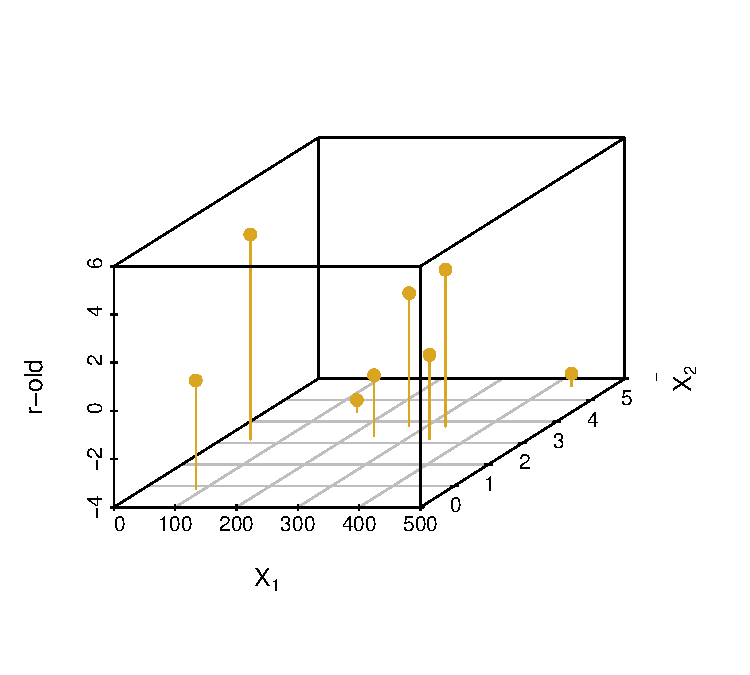
\includegraphics[scale=0.9]{scatterB.pdf}}
\end{center}

\vspace{-8mm}

\item Now that you have the prediction from the second weak learner, please compute the new residuals for each observation to find out where this learner did well and where it did poorly. Fill them in the column labeled \emph{$r_{new}$}.

\end{enumerate}

\newpage

\begin{center}
\textsc{Math 243: Statistical Learning} \\
\noindent\rule{12cm}{0.4pt}
\end{center}

\subsection*{Boosted Trees}

\emph{Third Weak Learner} ($b = 3$): We continue to strengthen our tree by incorporating a third weak learner that addresses the most glaring deficiencies of the first two learners.

\begin{enumerate}
\item The structure of the third weak learner is shown in the tree diagram below. Please fill in the prediction at each of the leaves as well as in the table in the column labeled $\hat{f}^3(x)$.

\vspace{10mm}

\begin{minipage}[t]{.4\textwidth}
{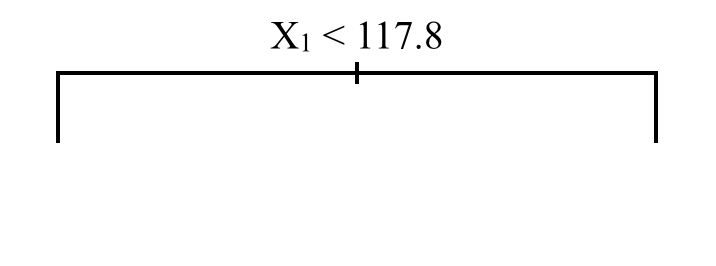
\includegraphics[width=\textwidth]{treeC.png}}
\end{minipage}
\hfill
\begin{minipage}[t]{.4\textwidth}
% latex table generated in R 3.2.3 by xtable 1.8-0 package
% Wed Mar 30 10:02:24 2016
\begin{tabular}{rrrrl}
  \hline
 & $X_1$ & $X_2$ & $r_{old}$ & $\hat{f}^3(x)$ \\ 
  \hline
1 & 270.00 & 3.81 & 0.33 &  \\ 
  2 & 86.03 & 0.86 & -0.67 &  \\ 
  3 & 149.53 & 4.44 & 0.00 &  \\ 
  4 & 331.15 & 3.77 & 1.33 &  \\ 
  5 & 430.89 & 5.68 & 0.00 &  \\ 
  6 & 338.36 & 3.18 & -1.67 &  \\ 
  7 & 46.33 & 3.17 & 3.33 &  \\ 
  8 & 238.19 & 3.35 & -2.67 &  \\ 
   \hline
\end{tabular}

\end{minipage}

\vspace{8mm}
\item Carefully draw the surface corresponding to $\hat{f}^3(x)$ on the 3D scatterplot below.

\vspace{-8mm}

\begin{center}
{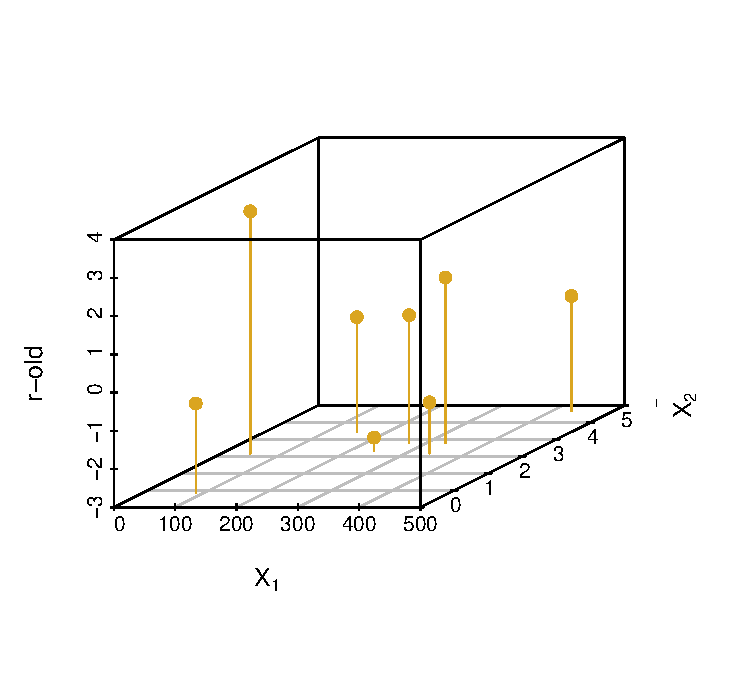
\includegraphics[scale=0.9]{scatterC.pdf}}
\end{center}

\end{enumerate}

\newpage

\begin{center}
\textsc{Math 243: Statistical Learning} \\
\noindent\rule{12cm}{0.4pt}
\end{center}

\subsection*{Boosted Trees}

\emph{Full Boosted Model}: Let's say we're sufficently satisfied with having three weak learners. The final step is to combine them into the final model.

\begin{enumerate}
\item Fill in the final boosted estimates, $\hat{f}^{boost}(x)$, in the table below.

\vspace{10mm}

% latex table generated in R 3.2.3 by xtable 1.8-0 package
% Wed Mar 30 10:02:25 2016
\begin{tabular}{rrrrrrrl}
  \hline
 & $X_1$ & $X_2$ & $Y$ & $\hat{f}^1(x)$ & $\hat{f}^2(x)$ & $\hat{f}^3(x)$ & $\hat{f}^{boost}(x)$ \\ 
  \hline
1 & 270.00 & 3.81 & 15.00 & 13.50 & 1.17 & -0.44 &  \\ 
  2 & 86.03 & 0.86 & 23.00 & 22.50 & 1.17 & 1.33 &  \\ 
  3 & 149.53 & 4.44 & 19.00 & 22.50 & -3.50 & -0.44 &  \\ 
  4 & 331.15 & 3.77 & 16.00 & 13.50 & 1.17 & -0.44 &  \\ 
  5 & 430.89 & 5.68 & 10.00 & 13.50 & -3.50 & -0.44 &  \\ 
  6 & 338.36 & 3.18 & 13.00 & 13.50 & 1.17 & -0.44 &  \\ 
  7 & 46.33 & 3.17 & 27.00 & 22.50 & 1.17 & 1.33 &  \\ 
  8 & 238.19 & 3.35 & 21.00 & 22.50 & 1.17 & -0.44 &  \\ 
   \hline
\end{tabular}


\vspace{8mm}
\item Carefully draw the surface corresponding to $\hat{f}^{boost}(x)$ on the 3D scatterplot below (yes, this is difficult!). Note that we're back to the same coordinates as in the scatterplot for the first weak learner.

\vspace{-8mm}

\begin{center}
{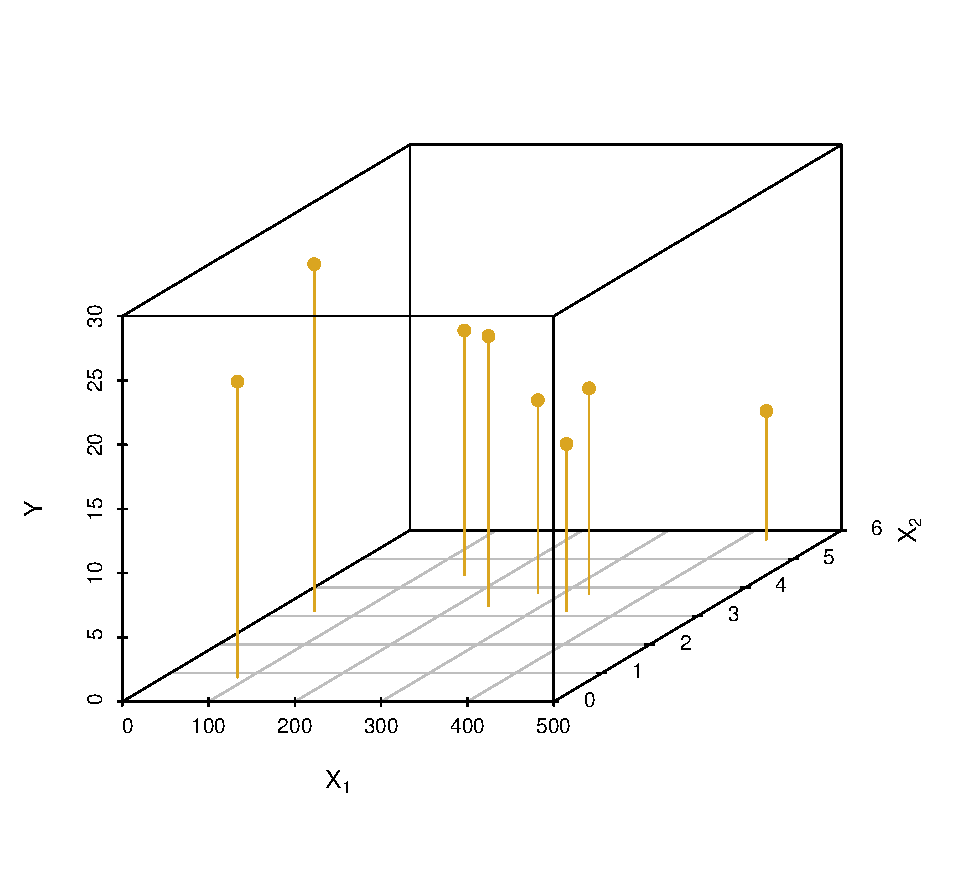
\includegraphics[scale=0.9]{scatterD.pdf}}
\end{center}


\newpage

\begin{center}
\textsc{Math 243: Statistical Learning} \\
\noindent\rule{12cm}{0.4pt}
\end{center}

\item What value did we use for $d$, the depth of each weak learner?
\vspace{8mm}

\item What value did we use for $B$, the number of weak learners?
\vspace{8mm}

\item What value did we use for $\lambda$, the shrinkage parameter?
\vspace{8mm}

\item Please describe the trend in the amount of explanatory power of each successive learner, $\hat{f}^1(x)$ to $\hat{f}^3(x)$.
\vspace{25mm}

\item What would be the consequences if we set $\lambda = 0.01$?
\vspace{8mm}

\end{enumerate}


\end{document}
